\documentclass[12pt]{article}

\usepackage[english]{babel}
\usepackage{xcolor}
\usepackage{blindtext}
\usepackage{graphicx}
\usepackage{amssymb}
\usepackage{amsthm}
\usepackage{amsmath}
\usepackage{bbold}
\usepackage{bm}
\usepackage{physics}
\usepackage[a4paper, width = 185mm, top = 15mm, bottom = 15mm]{geometry}
\usepackage{calligra}
\usepackage{tikz-feynman}
\usepackage{pdflscape}

\tikzset{graviton/.style={decorate, decoration={snake, amplitude=.4mm, segment length=1.9mm, pre length=.5mm, post length=.5mm}, double}}



\DeclareMathAlphabet{\mathcalligra}{T1}{calliga}{m}{n}
\DeclareFontShape{T1}{calligra}{m}{n}{<->s*[2.2]callig15}{}

\newcommand{\scripty}[1]{\ensuremath{\mathcalligra{#1}}}
\renewcommand* \d{\mathop{}\!\mathrm{d}}



\begin{document}
\noindent
A general Green function is given by:
\begin{equation}
G_{ab}^{\sigma\sigma'}(i\omega_n)=
\vcenter{\hbox{
  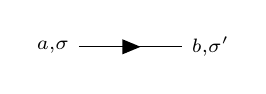
\begin{tikzpicture}
    \begin{feynman}
      \vertex (a) at (0,0) {\(\scriptstyle a, \sigma\)};
      \vertex[right=2cm of a] (b) {\(\scriptstyle b,\sigma'\)};
      \diagram* {
        (a) -- [fermion] (b),
      };
    \end{feynman}
  \end{tikzpicture}
}}
\end{equation}
Here $a$ and $b$ are spacial indices which would run from 0 to 1 in the case for the Hubbard dimer. In this case the Green function doesn't flip spin:
\begin{equation}
\delta_{\sigma\sigma'}G_{ab}^{\sigma\sigma'}= G_{ab}^{\sigma}(i\omega_n)=
\vcenter{\hbox{
  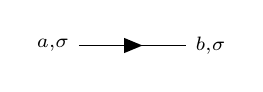
\begin{tikzpicture}
    \begin{feynman}
      \vertex (a) at (0,0) {\(\scriptstyle a, \sigma\)};
      \vertex[right=2cm of a] (b) {\(\scriptstyle b,\sigma\)};
      \diagram* {
        (a) -- [fermion] (b),
      };
    \end{feynman}
  \end{tikzpicture}
}}
\end{equation}
For the polarization we have:
\begin{equation}
P_{abcd}^{\sigma\sigma'\sigma''\sigma'''}(i\omega_n) =
\vcenter{\hbox{
  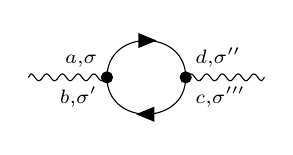
\begin{tikzpicture}
    \begin{feynman}
      \vertex (a);
      \vertex[right=1cm of a] (b);
      \vertex[left=1cm of a] (c);
      \vertex[right=1cm of b] (d);
      \diagram* {
        (a) -- [fermion, half left, looseness=1.6] (b),
        (b) -- [fermion, half left, looseness=1.6] (a),
        (a) -- [photon] (c),
        (b) -- [photon] (d)
      };
      \filldraw (a) circle (2pt);
       \filldraw (b) circle (2pt);
    \end{feynman}
    \node [above left] at (a) {\(\scriptstyle a,\sigma\)};
    \node [below left] at (a) {\(\scriptstyle b,\sigma'\)};
    
    \node [above right] at (b) {\(\scriptstyle d,\sigma''\)};
    \node [below right] at (b) {\(\scriptstyle c,\sigma'''\)};
    
  \end{tikzpicture}
}}
\end{equation}
But we know the Green functions don't change spin so we get:
\begin{equation}
\delta_{\sigma\sigma''}\delta_{\sigma'\sigma'''} P_{abcd}^{\sigma\sigma'\sigma''\sigma'''}(i\omega_n) =P_{abcd}^{\sigma\sigma'\sigma'\sigma}(i\omega_n)=P_{abcd}^{\sigma\sigma'}(i\omega_n)=
\vcenter{\hbox{
  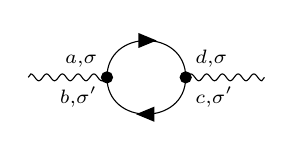
\begin{tikzpicture}
    \begin{feynman}
      \vertex (a);
      \vertex[right=1cm of a] (b);
      \vertex[left=1cm of a] (c);
      \vertex[right=1cm of b] (d);
      \diagram* {
        (a) -- [fermion, half left, looseness=1.6] (b),
        (b) -- [fermion, half left, looseness=1.6] (a),
        (a) -- [photon] (c),
        (b) -- [photon] (d)
      };
      \filldraw (a) circle (2pt);
       \filldraw (b) circle (2pt);
    \end{feynman}
    \node [above left] at (a) {\(\scriptstyle a,\sigma\)};
    \node [below left] at (a) {\(\scriptstyle b,\sigma'\)};
    
    \node [above right] at (b) {\(\scriptstyle d,\sigma\)};
    \node [below right] at (b) {\(\scriptstyle c,\sigma'\)};
    
  \end{tikzpicture}
}}
\end{equation}
And in terms of the Green functions we have:
$$P_{abcd}^{\sigma\sigma'}(i\omega_n)=-\mathcal{F}_{\tau\to i\omega_n}\{G_{da}^{\sigma}(\tau)G_{bc}^{\sigma'}(-\tau)\}$$
Note that the polarization is just the bubble diagram and without the Coulomb lines which would enforce additional restrictions as shown now. For the Coulomb interaction we have:
\begin{equation}
V_{abcd}^{\sigma\sigma'\sigma''\sigma'''}=
\vcenter{\hbox{
  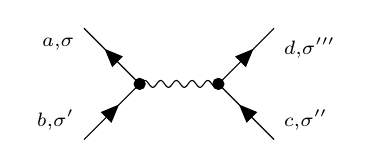
\begin{tikzpicture}
    \begin{feynman}
      \vertex (a);
      \vertex[right=1cm of a] (b);
      \vertex[above left=1cm of a] (c);
      \vertex[below left=1cm of a] (d);
      \vertex[below right=1cm of b] (e);
      \vertex[above right=1cm of b] (f);
      \diagram* {
        (a) -- [photon] (b),
        (a) -- [fermion] (c),
        (d) -- [fermion] (a),
        (e) -- [fermion] (b),
        (b) -- [fermion] (f),
      };
      \filldraw (a) circle (2pt);
       \filldraw (b) circle (2pt);
    \end{feynman}
    \node [below left] at (c) {\(\scriptstyle a,\sigma\)};
    \node [above left] at (d) {\(\scriptstyle b,\sigma'\)};
    
    \node [below right] at (f) {\(\scriptstyle d,\sigma'''\)};
    \node [above right] at (e) {\(\scriptstyle c,\sigma''\)};
    
  \end{tikzpicture}
}}
\end{equation}
And if we say that the Coulomb interaction doesn't change spin we get:
\begin{equation}
\delta_{\sigma\sigma'}\delta_{\sigma''\sigma'''} V_{abcd}^{\sigma\sigma'\sigma''\sigma'''}=V_{abcd}^{\sigma\sigma\sigma''\sigma''}=V_{abcd}^{\sigma\sigma'}=
\vcenter{\hbox{
  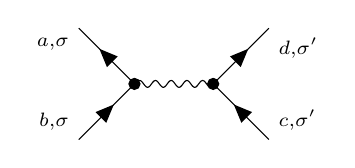
\begin{tikzpicture}
    \begin{feynman}
      \vertex (a);
      \vertex[right=1cm of a] (b);
      \vertex[above left=1cm of a] (c);
      \vertex[below left=1cm of a] (d);
      \vertex[below right=1cm of b] (e);
      \vertex[above right=1cm of b] (f);
      \diagram* {
        (a) -- [photon] (b),
        (a) -- [fermion] (c),
        (d) -- [fermion] (a),
        (e) -- [fermion] (b),
        (b) -- [fermion] (f),
      };
      \filldraw (a) circle (2pt);
       \filldraw (b) circle (2pt);
    \end{feynman}
    \node [below left] at (c) {\(\scriptstyle a,\sigma\)};
    \node [above left] at (d) {\(\scriptstyle b,\sigma\)};
    
    \node [below right] at (f) {\(\scriptstyle d,\sigma'\)};
    \node [above right] at (e) {\(\scriptstyle c,\sigma'\)};
    
  \end{tikzpicture}
}}
\end{equation}
For the screened interaction we then get:
\begin{align}
W_{abcd}^{\sigma\sigma'\sigma''\sigma'''}(i\omega_n)=&\ V_{abcd}^{\sigma\sigma'\sigma''\sigma'''}+
\sum_{\sigma_1\sigma_2\sigma_3\sigma_4}\sum_{abcd}V_{abef}^{\sigma\sigma'\sigma_3\sigma_4}\Pi_{fegh}^{\sigma_2\sigma_1\sigma_3\sigma_4}(i\omega_n)W_{hgcd}^{\sigma_4\sigma_3\sigma''\sigma'''}(i\omega_n)\\
=&\ \delta_{\sigma\sigma'}\delta_{\sigma''\sigma'''}V_{abcd}^{\sigma\sigma'\sigma''\sigma'''}\\
&+
\sum_{\sigma_1\sigma_2\sigma_3\sigma_4}\sum_{abcd}\delta_{\sigma\sigma'}\delta_{\sigma_3\sigma_4}V_{abef}^{\sigma\sigma'\sigma_3\sigma_4}\delta_{\sigma_2\sigma_3}\delta_{\sigma_1\sigma_4}\Pi_{fegh}^{\sigma_2\sigma_1\sigma_3\sigma_4}(i\omega_n)W_{hgcd}^{\sigma_4\sigma_3\sigma''\sigma'''}(i\omega_n)\\
=&\ V_{abcd}^{\sigma\sigma\sigma''\sigma''}+
\sum_{\sigma_1}\sum_{abcd}V_{abef}^{\sigma\sigma\sigma_1\sigma_1}\Pi_{fegh}^{\sigma_1\sigma_1\sigma_1\sigma_1}(i\omega_n)W_{hgcd}^{\sigma_1\sigma_1\sigma''\sigma'''}(i\omega_n)\\
W_{abcd}^{\sigma\sigma'}(i\omega_n)=&\ V_{abcd}^{\sigma\sigma'}+
\sum_{\sigma_1}\sum_{abcd}V_{abef}^{\sigma\sigma_1}\Pi_{fegh}^{\sigma_1}(i\omega_n)W_{hgcd}^{\sigma_1\sigma'}(i\omega_n)
\end{align}
So in a spin full calculation, we have to explicitly sum over the spin when calculating the screened potential and if spin is not taken into account, the polarization diagram has a symmetry which results in a factor two. In our case with the Hubbard dimer, the two spin blocks are identical so we end up with this same factor of 2, explaining my earlier results. But this does raise the question on whether or not to include this factor for the Hartree contribution for the self energy. TPRF's GW solver doesn't take this into account so nor will I for comparison but this is something to think about.
\newpage
\noindent
For the Green function I'll use the following convention:
\begin{equation}
G_{ij}^{\sigma}(i\omega_n)=
\vcenter{\hbox{
  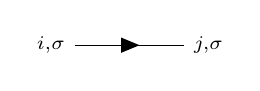
\begin{tikzpicture}
    \begin{feynman}
      \vertex (a) at (0,0) {\(\scriptstyle i, \sigma\)};
      \vertex[right=2cm of a] (b) {\(\scriptstyle j,\sigma\)};
      \diagram* {
        (a) -- [fermion] (b),
      };
    \end{feynman}
  \end{tikzpicture}
}}
\end{equation}
Which carries only one spin index because we're only considering processes that don't flip the spin. For the Coulomb interaction I'll use the following convention:
\begin{equation}
V_{ijkl}^{\sigma\sigma'}=
\vcenter{\hbox{
  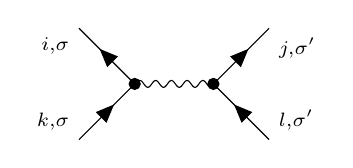
\begin{tikzpicture}
    \begin{feynman}
      \vertex (a);
      \vertex[right=1cm of a] (b);
      \vertex[above left=1cm of a] (c);
      \vertex[below left=1cm of a] (d);
      \vertex[below right=1cm of b] (e);
      \vertex[above right=1cm of b] (f);
      \diagram* {
        (a) -- [photon] (b),
        (a) -- [fermion] (c),
        (d) -- [fermion] (a),
        (e) -- [fermion] (b),
        (b) -- [fermion] (f),
      };
      \filldraw (a) circle (2pt);
       \filldraw (b) circle (2pt);
    \end{feynman}
    \node [below left] at (c) {\(\scriptstyle i,\sigma\)};
    \node [above left] at (d) {\(\scriptstyle k,\sigma\)};
    
    \node [below right] at (f) {\(\scriptstyle j,\sigma'\)};
    \node [above right] at (e) {\(\scriptstyle l,\sigma'\)};
    
  \end{tikzpicture}
}}
\end{equation}
Which is consistent with:
\begin{equation}
\hat{V}=\dfrac{1}{2}\sum_{\sigma\sigma'}\sum_{ijkl}V_{ijkl}^{\sigma\sigma'}\hat{a}_{i\sigma}^\dagger\hat{a}_{j\sigma'}^\dagger\hat{a}_{l\sigma'}\hat{a}_{k\sigma}
\end{equation}
For the screened interaction we have:
\begin{align}
W_{ijkl}^{\sigma\sigma'}=
\vcenter{\hbox{
  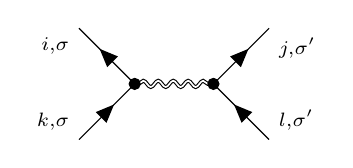
\begin{tikzpicture}
    \begin{feynman}
      \vertex (a);
      \vertex[right=1cm of a] (b);
      \vertex[above left=1cm of a] (c);
      \vertex[below left=1cm of a] (d);
      \vertex[below right=1cm of b] (e);
      \vertex[above right=1cm of b] (f);
      \diagram* {
        (a) -- [graviton] (b),
        (a) -- [fermion] (c),
        (d) -- [fermion] (a),
        (e) -- [fermion] (b),
        (b) -- [fermion] (f),
      };
      \filldraw (a) circle (2pt);
       \filldraw (b) circle (2pt);
    \end{feynman}
    \node [below left] at (c) {\(\scriptstyle i,\sigma\)};
    \node [above left] at (d) {\(\scriptstyle k,\sigma\)};    
    \node [below right] at (f) {\(\scriptstyle j,\sigma'\)};
    \node [above right] at (e) {\(\scriptstyle l,\sigma'\)};    
  \end{tikzpicture}
}}&=\vcenter{\hbox{
  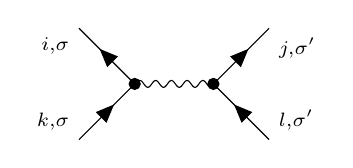
\begin{tikzpicture}
    \begin{feynman}
      \vertex (a);
      \vertex[right=1cm of a] (b);
      \vertex[above left=1cm of a] (c);
      \vertex[below left=1cm of a] (d);
      \vertex[below right=1cm of b] (e);
      \vertex[above right=1cm of b] (f);
      \diagram* {
        (a) -- [photon] (b),
        (a) -- [fermion] (c),
        (d) -- [fermion] (a),
        (e) -- [fermion] (b),
        (b) -- [fermion] (f),
      };
      \filldraw (a) circle (2pt);
       \filldraw (b) circle (2pt);
    \end{feynman}
    \node [below left] at (c) {\(\scriptstyle i,\sigma\)};
    \node [above left] at (d) {\(\scriptstyle k,\sigma\)};
    \node [below right] at (f) {\(\scriptstyle j,\sigma'\)};
    \node [above right] at (e) {\(\scriptstyle l,\sigma'\)}; 
  \end{tikzpicture}
}}+\vcenter{\hbox{
  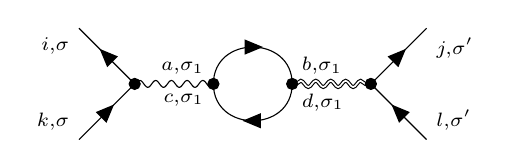
\begin{tikzpicture}
    \begin{feynman}
      \vertex (a);
      \vertex[right=1cm of a] (b);
      \vertex[above left=1cm of a] (c);
      \vertex[below left=1cm of a] (d);
      \vertex[right=1cm of b] (e);
      \vertex[right=1cm of e] (f);
      \vertex[above right=1cm of f] (g);
      \vertex[below right=1cm of f] (h);
      \diagram* {
        (a) -- [photon] (b),
        (a) -- [fermion] (c),
        (d) -- [fermion] (a),
        (b) -- [fermion, half left, looseness=1.6] (e),
        (e) -- [fermion, half left, looseness=1.6] (b),
        (e) -- [graviton] (f),
        (f) -- [fermion] (g),
        (h) -- [fermion] (f),
      };
      \filldraw (a) circle (2pt);
       \filldraw (b) circle (2pt);
       \filldraw (e) circle (2pt);
       \filldraw (f) circle (2pt);
    \end{feynman}
    \node [below right] at (g) {\(\scriptstyle j,\sigma'\)};
    \node [above right] at (h) {\(\scriptstyle l,\sigma'\)};
    \node [below left] at (c) {\(\scriptstyle i,\sigma\)};
    \node [above left] at (d) {\(\scriptstyle k,\sigma\)};
    \node [above left] at (b) {\(\scriptstyle a,\sigma_1\)};
    \node [below left] at (b) {\(\scriptstyle c,\sigma_1\)};  
    \node [above right] at (e) {\(\scriptstyle b,\sigma_1\)};
    \node [below right] at (e) {\(\scriptstyle d,\sigma_1\)}; 
  \end{tikzpicture}
}}\\
&=V_{ijkl}^{\sigma\sigma'} + \sum_{\sigma_1}\sum_{abcd} V_{iakc}^{\sigma\sigma_1}P_{acbd}^{\sigma_1}W_{cjbl}^{\sigma_1\sigma'}
\end{align}
Where the polarization is now defined as:
\begin{equation}
P_{abcd}^{\sigma}\propto G_{ac}^{\sigma}G_{db}^\sigma
\end{equation}
For the self energy we have:
\begin{align}
\Sigma_{ij}^{\sigma}&=  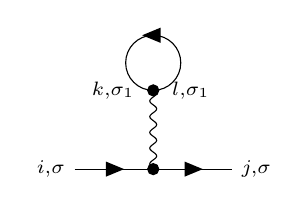
\begin{tikzpicture}[baseline=-3]
    \begin{feynman}
      \vertex (a) {\(\scriptstyle i, \sigma\)};
      \vertex[right=1.3cm of a] (b);
		\vertex[right=1cm of b] (c){\(\scriptstyle j, \sigma\)};
		\vertex[above=1cm of b] (d);
		\vertex[above=0.7cm of d] (e);
		\vertex[left=0.02cm of e] (g);
      \diagram* {
        (a) -- [fermion] (b),
        (b) -- [fermion] (c),
        (b) -- [photon] (d),
        (e) -- [fermion] (g),
      };
      \filldraw (b) circle (2pt);
      \filldraw (d) circle (2pt);
       \draw (d) arc(-90:270:0.35);
       \node [right] at (d) {\(\ \scriptstyle l,\sigma_1\)}; 
       \node [left] at (d) {\(\scriptstyle k,\sigma_1 \ \)}; 
    \end{feynman} 
  \end{tikzpicture} +
  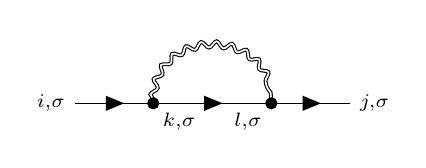
\begin{tikzpicture}[baseline=-3]
    \begin{feynman}
      \vertex (a) {\(\scriptstyle i, \sigma\)};
      \vertex[right=1.3cm of a] (b);
		\vertex[right=1.5cm of b] (c);
		\vertex[right=1cm of c] (d){\(\scriptstyle j, \sigma\)};
      \diagram* {
        (a) -- [fermion] (b),
        (b) -- [fermion] (c),
        (c) -- [fermion] (d),
        (b) -- [graviton, half left, looseness=1.6] (c)
      };
      \filldraw (b) circle (2pt);
       \filldraw (c) circle (2pt);
       \node [below right] at (b) {\(\scriptstyle k,\sigma\)};
       \node [below left] at (c) {\(\scriptstyle l,\sigma\)};  
    \end{feynman} 
  \end{tikzpicture}\\
  &\propto \sum_{\sigma_1}\sum_{kl} V_{ljki}^{\sigma\sigma_1}G_{lk}^{\sigma_1} + W_{jkli}^{\sigma\sigma}G_{kl}^{\sigma}
\end{align}
Where the first term is the Hartree term and the second term can be split up into a dynamical part and the Fock term by splitting $W\to (W-V) + V$. And we can also see that for calculating the self energy, we only need the spin diagonal components of the screened potential.
\newpage
\noindent
Assuming the Coulomb interactions do not scatter, i.e. they don't change the position of an electron as well as preserve spin, we can instead write $V_{ijkl}^{\sigma\sigma'}$ as a two index object: $V_{ij}^{\sigma\sigma'}=V_{ijij}^{\sigma\sigma'}$, the same goes for $W$ and for $P$. This simplifies our equations to:
\begin{align}
W_{ij}^{\sigma\sigma'}&=V_{ij}^{\sigma\sigma'}+\sum_{\sigma_1,kl}V_{ik}^{\sigma\sigma_1}P_{kl}^{\sigma_1}W_{kj}^{\sigma_1\sigma'}\\
\tilde{\Sigma}_{ij}^{\sigma}&=\tilde{W}_{ij}^{\sigma\sigma}G_{ij}^{\sigma}\\
\Sigma_{ij}^{\sigma, \text{Fock}}&=V_{ij}^{\sigma\sigma}G_{ij}^{\sigma}\\
\Sigma_{ii}^{\sigma, \text{Hartree}}&=\sum_{\sigma_1, j}V_{ij}^{\sigma\sigma_1}G_{jj}^{\sigma_1}
\end{align}
\end{document}